%%% template.tex
%%%
%%% This LaTeX source document can be used as the basis for your technical
%%% paper or abstract. Intentionally stripped of annotation, the parameters
%%% and commands should be adjusted for your particular paper - title, 
%%% author, article DOI, etc.
%%% The accompanying ``template.annotated.tex'' provides copious annotation
%%% for the commands and parameters found in the source document. (The code
%%% is identical in ``template.tex'' and ``template.annotated.tex.'')

\documentclass[]{acmsiggraph}
\usepackage{algorithm}
\usepackage[noend]{algpseudocode}
\TOGonlineid{45678}
\TOGvolume{0}
\TOGnumber{0}
\TOGarticleDOI{0}
\TOGprojectURL{}
\TOGvideoURL{}
\TOGdataURL{}
\TOGcodeURL{}
\usepackage{color}
%\definecolor{red}{rgb}{0.9, 0.17, 0.31}
\usepackage{multirow}
\usepackage{subfig}
\usepackage{xcolor}
\usepackage{lipsum}
\usepackage{listings}
\usepackage{graphicx}
\usepackage{glsllst} % My own package providing markup listing for glsl
\usepackage{rmlst}   % My own package providing markup listing for renderman
\usepackage{amsmath}
\usepackage{hyperref}

\lstset{
	backgroundcolor=\color[rgb]{0.95, 0.95, 0.95},
	tabsize=3,
	%rulecolor=,
	basicstyle=\footnotesize\ttfamily,
	upquote=true,
	aboveskip={1.5\baselineskip},
	columns=fixed,
	showstringspaces=false,
	extendedchars=true,
	breaklines=true,
	prebreak = \raisebox{0ex}[0ex][0ex]{\ensuremath{\hookleftarrow}},
	frame=none,
	aboveskip=15pt,
	belowskip=8pt,
	captionpos=t,
	showtabs=false,
	showspaces=false,
	showstringspaces=false,
	identifierstyle=\ttfamily,
	%keywordstyle=\color{red}\bfseries,
	%keywordstyle=[1]\bfseries\color{syntaxBlue},
	%keywordstyle=[2]\bfseries\color{syntaxRed},
	%keywordstyle=[3]\color{blue}\bfseries,
	%keywordstyle=[4]\bfseries\color{syntaxBlue},
	commentstyle=\color[rgb]{0.082,0.639,0.082},
	keywordstyle=[1]\bfseries\color[rgb]{0,0,0.75},
	keywordstyle=[2]\bfseries\color[rgb]{0.5,0.0,0.0},
	keywordstyle=[3]\bfseries\color[rgb]{0.127,0.427,0.514},
	keywordstyle=[4]\bfseries\color[rgb]{0.4,0.4,0.4},
	stringstyle=\color[rgb]{0.639,0.082,0.082},
}

\title{Principles of Rendering: Real-time rendering}

\author{Callum Glover\thanks{e-mail:s4907224@bournemouth.ac.uk}\\National Centre for Computer Animation}
\pdfauthor{Callum Glover}

\keywords{rendering}

\begin{document}

\maketitle

\begin{abstract}
The purpose of this report is to document how I utilised GLSL through C++ to create a photorealistic shaded model of a Sandisk USB memory stick, using my previous work with OSL and Renderman as a 
basis to improve and iterate upon.  
\end{abstract}

\section{Introduction} \label{sec:Introduction}
\begin{figure}[htbp]\centering
 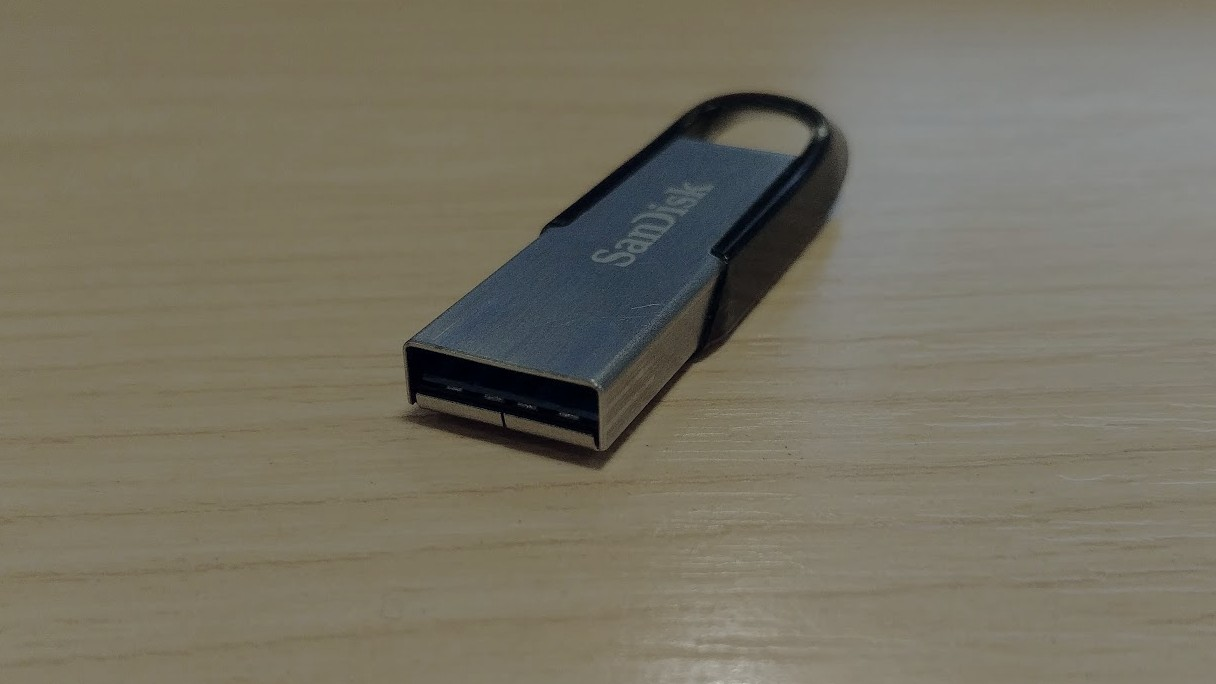
\includegraphics[width=0.75\linewidth]{images/pref.jpg}
 \caption{\label{fig:reference}The original reference image.}
\end{figure}

\begin{figure}[htbp]\centering
 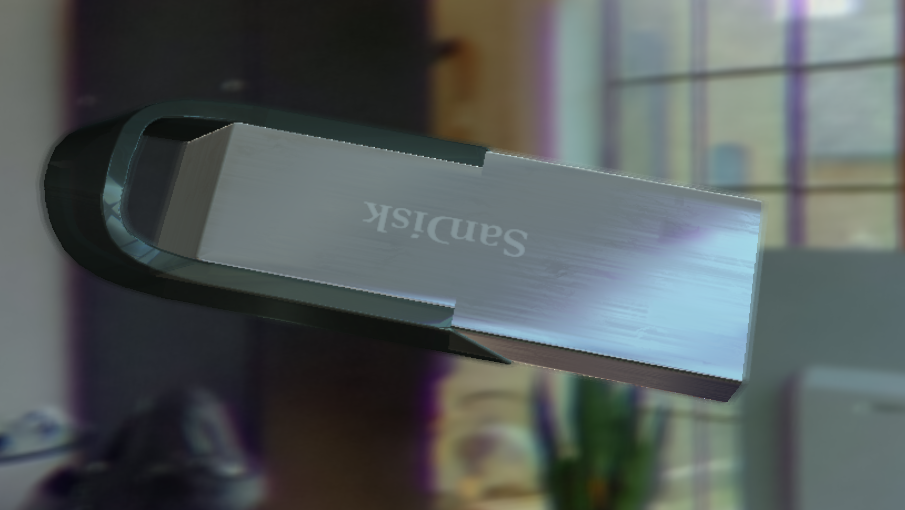
\includegraphics[width=0.75\linewidth]{images/tempRef.png}
 \caption{\label{fig:final}The final rendered image.}
\end{figure}

By analysing the object, the shader would break into the following properties:
\begin{enumerate}    
    \item The main metal surfaces have brushed marks, resulting in varying roughness over the surface and also small differences in the angle of reflected light.
    \item The surfaces have defined highlights on the rounded edges, and wider highlights over the larger surfaces.
    \item There are small scratches on the surfaces that seem less rough than their surrounding areas, leading to differently shaped highlights.
    \item There is an etched logo in the centre, with a higher roughness than the rest of the surface.
    \item Other than the logo, the memory stick seems to have a uniform material colour.
    \item The innards of the memory stick are relatively uniform in appearance, constiting of blue plastic with a black plastic underlay, and gold contacts on top.
    \item The gold contacts on top of the blue plastic are highly metallic, leading to large highlights when lit, however almost black when out of light.
    \item There is a translucent plastic surround to the metal housing that has wide specular highlights that clearly reflect the environment.
    \item The plastic is not overly transparent, and so from many angles it appears nearly entirely reflective.
\end{enumerate}

\section{Method} \label{sec:Method}
To start development of shaders, I initially created the base model in Maya, making sure to properly UV the object so later noise application worked as intended.  After instancing the model into 
an OpenGL context I started development of the base PBR shader that I would modify for the individual components of the object.  At first the shader used the Beckmann distribution for the specular 
component, though I switched to using GGX for aesthetic reasons, as it generally led to wider highlights on the metal surfaces. ***You should stick an image of that here***

I then worked on expanding my shader to work with environment lighting by passing through a set of pre-defined lights for lighting calculations, and an environment cubemap for the specular colour.
I encountered issues with deciding how to calculate the view vector, as I was working with the mindset of using the camera's rotation to rotate the object rather than to rotate around the object, 
and as such I had thought a constant view vector down the Z axis would make sense.  Unfortunately due to the flat nature of the main housing, the reflection vector would be the same for all fragments 
adjacent to each other on a flat surface, and so I came to the realisation the view vector would simply be the normalised, negative position of the fragment in unprojected eye space, as the cubemap 
is also handled via unprojected space.

The environment cube itself is simply a cube that the camera sits in, using the eye space fragment position of the cube as a lookup vector to the sampler.

As the memory stick is comprised of mutliple different elements with differing properties, I separated the mesh into groups of the same material, and created a USB structure to hold the meshes and 
their respective shaders and properties.  I modified the base PBR shader to take in $roughness$, $metallic$, $diffuse$ and $specular$ colour and multipliers along with $alpha$ for transparency 
handling, all of which I defined in the USB structure.


\section{Results} \label{sec:Results}
Results text \cite{blenderSushi}

\bibliographystyle{acmsiggraph}
\bibliography{references}




\end{document}

